% =====================================================================
% CHAPTER 6 & 7: RESULTS, EVALUATION, AND CONCLUSION
% =====================================================================

\section{ EXPERIMENTAL RESULTS AND EVALUATION}
\addcontentsline{toc}{section}{CHAPTER 6. EXPERIMENTAL RESULTS AND EVALUATION}
\subsection{Model Comparison with Default Hyperparameters}

\noindent\textbf{Table 6.1} 5-fold cross-validation results on the training set (averaged across folds, default hyperparameters, 0.50 threshold), sorted by F1.

\begin{center}
\small
\begin{tabular}{l r r r r r r r}
\toprule
\textbf{Model} & \textbf{Accuracy} & \textbf{Precision} & \textbf{Recall} & \textbf{F1} & \textbf{ROC-AUC} & \textbf{PR-AUC} & \textbf{F1 Std} \\
\midrule
Logistic Regression & 0.803 & 0.655 & 0.546 & \textbf{0.595} & 0.846 & 0.660 & 0.023 \\
AdaBoost & 0.804 & 0.670 & 0.521 & 0.586 & 0.849 & 0.666 & 0.010 \\
Gradient Boosting & 0.801 & 0.662 & 0.511 & 0.576 & 0.848 & 0.664 & 0.016 \\
KNN & 0.782 & 0.597 & 0.553 & 0.574 & 0.818 & 0.572 & 0.025 \\
Random Forest & 0.793 & 0.645 & 0.496 & 0.561 & 0.827 & 0.631 & 0.015 \\
Decision Tree & 0.733 & 0.497 & 0.514 & 0.505 & 0.663 & 0.385 & 0.019 \\
Dummy Baseline & 0.608 & 0.265 & 0.268 & 0.266 & 0.499 & 0.266 & 0.020 \\
\bottomrule
\end{tabular}
\end{center}

Key observations:

\begin{itemize}
    \item \textbf{All models outperform the baseline.} Dummy achieved an ROC-AUC of 0.499 (exact random level) and PR-AUC of 0.266 (exact positive class ratio), confirming no obvious evaluation bugs and that the data genuinely contains predictive signals.
    \item \textbf{The top four models perform comparably in ranking ability.} LR, AdaBoost, and Gradient Boosting achieved ROC-AUCs between 0.846–0.849 and PR-AUCs of 0.660–0.666; differences are smaller than fold-to-fold F1 standard deviations (0.010–0.025). LR ranking first in F1 at this stage is insufficient to declare it superior.
    \item \textbf{Recall at the 0.50 threshold is low.} Most models achieved a Recall of only 0.50–0.55, missing about half of departing customers despite ~0.80 accuracy. This is a typical symptom of models leaning toward the majority class under class imbalance, motivating the use of \texttt{class\_weight} and threshold tuning.
    \item \textbf{Unconstrained Decision Tree overfits.} ROC-AUC was only 0.663 and PR-AUC 0.385, significantly lower than ensemble models, consistent with single trees memorizing training data.
    \item \textbf{AdaBoost achieved the highest ROC-AUC and PR-AUC but ranked second in F1}, due to high Precision (0.670) paired with low Recall (0.521) at threshold 0.50. This indicates fixed-threshold F1 and threshold-independent metrics can rank models differently.
\end{itemize}

\subsection{ Results After Hyperparameter Tuning}

\noindent\textbf{Table 6.2} Best cross-validation F1 after GridSearchCV and corresponding configurations (threshold 0.50).

\begin{center}
\small
\begin{tabularx}{\textwidth}{l r r r r X}
\toprule
\textbf{Model} & \textbf{Default F1} & \textbf{Tuned F1} & \textbf{Gain} & \textbf{F1 Std} & \textbf{Best Configuration} \\
\midrule
Random Forest & 0.561 & \textbf{0.636} & +0.075 & 0.006 & \texttt{class\_weight = balanced}; \texttt{max\_depth = 10}; \texttt{min\_samples\_leaf = 5}; \texttt{n\_estimators = 100} \\
\addlinespace
Logistic Regression & 0.595 & 0.634 & +0.039 & 0.008 & \texttt{C = 0.5}; \texttt{class\_weight = balanced} \\
\addlinespace
Decision Tree & 0.505 & 0.607 & +0.102 & 0.009 & \texttt{class\_weight = balanced}; \texttt{max\_depth = 5}; \texttt{min\_samples\_leaf = 10} \\
\addlinespace
KNN & 0.574 & 0.598 & +0.024 & 0.015 & \texttt{n\_neighbors = 31}; \texttt{p = 1}; \texttt{weights = uniform} \\
\addlinespace
Gradient Boosting & 0.576 & 0.586 & +0.010 & 0.022 & \texttt{learning\_rate = 0.08}; \texttt{max\_depth = 3}; \texttt{n\_estimators = 200} \\
\addlinespace
AdaBoost & 0.586 & 0.586 & +0.000 & 0.010 & \texttt{learning\_rate = 1.0}; \texttt{n\_estimators = 100} \\
\bottomrule
\end{tabularx}
\end{center}

Key observations:

\begin{itemize}
    \item \textbf{\texttt{class\_weight = "balanced"} is the primary driver of performance gains.} All three models supporting this parameter (Random Forest, Logistic Regression, Decision Tree) selected "balanced", achieving the largest F1 gains (+0.075, +0.039, +0.102). Conversely, AdaBoost and Gradient Boosting lacked this parameter and showed virtually no improvement (+0.000 and +0.010). Thus, most tuning benefits stemmed from handling class imbalance rather than increasing model complexity.
    \item \textbf{Random Forest was selected, but its margin over Logistic Regression is negligible.} RF achieved an F1 of 0.636 versus 0.634 for LR; the 0.002 gap is smaller than cross-validation standard deviations (0.006–0.008), meaning the two models are statistically indistinguishable. Following preset rules (highest cross-validation F1), Random Forest was chosen; if interpretability is prioritized, Logistic Regression serves as a sound alternative with equivalent performance.
    \item \textbf{GridSearchCV peak scores exhibit slight optimistic bias}, being selected as maximum values across multiple configurations on the same data. Final figures therefore require confirmation on a held-out test set (Section 6.4).
\end{itemize}

\subsection{ Classification Threshold Selection}

Based on out-of-fold training probabilities, the threshold maximizing F1 was \textbf{$t = 0.46$}, with $\text{F1} = 0.639$. This value is merely 0.003 higher than the cross-validation F1 at threshold 0.50 (0.636; noting differing calculation methods between fold averaging and pooled out-of-fold predictions), indicating that the F1-threshold curve is relatively flat around 0.50. A slightly lower threshold makes the model more inclined to label instances as "departed", increasing Recall while slightly lowering Precision.

\subsection{ Evaluation on the Test Set}

\noindent\textbf{Table 6.3} Results of the tuned Random Forest on the test set (1,407 records).

\begin{center}
\small
\begin{tabular}{l r r r r r r}
\toprule
\textbf{Threshold} & \textbf{Accuracy} & \textbf{Precision} & \textbf{Recall} & \textbf{F1} & \textbf{ROC-AUC} & \textbf{PR-AUC} \\
\midrule
0.50 (default) & 0.758 & 0.531 & 0.767 & 0.628 & 0.838 & 0.639 \\
0.46 (selected) & 0.750 & 0.519 & 0.807 & \textbf{0.632} & 0.838 & 0.639 \\
\bottomrule
\end{tabular}
\end{center}

\vspace{0.5em}
\noindent\textbf{Table 6.4} Confusion matrix at threshold 0.46 (rows: actual labels; columns: predicted labels).

\begin{center}
\small
\begin{tabular}{l l l r}
\toprule
 & \textbf{Predicted: Stayed} & \textbf{Predicted: Departed} & \textbf{Total} \\
\midrule
\textbf{Actual: Stayed} & TN = 753 & FP = 280 & 1,033 \\
\textbf{Actual: Departed} & FN = 72 & TP = 302 & 374 \\
\bottomrule
\end{tabular}
\end{center}

\vspace{0.5em}
\noindent\textbf{Table 6.5} Classification report at threshold 0.46.

\begin{center}
\small
\begin{tabular}{l r r r r}
\toprule
\textbf{Class} & \textbf{Precision} & \textbf{Recall} & \textbf{F1} & \textbf{Sample Count} \\
\midrule
Stayed & 0.913 & 0.729 & 0.811 & 1,033 \\
Departed & 0.519 & 0.807 & 0.632 & 374 \\
Macro average & 0.716 & 0.768 & 0.721 & 1,407 \\
Weighted average & 0.808 & 0.750 & 0.763 & 1,407 \\
\bottomrule
\end{tabular}
\end{center}

\begin{center}
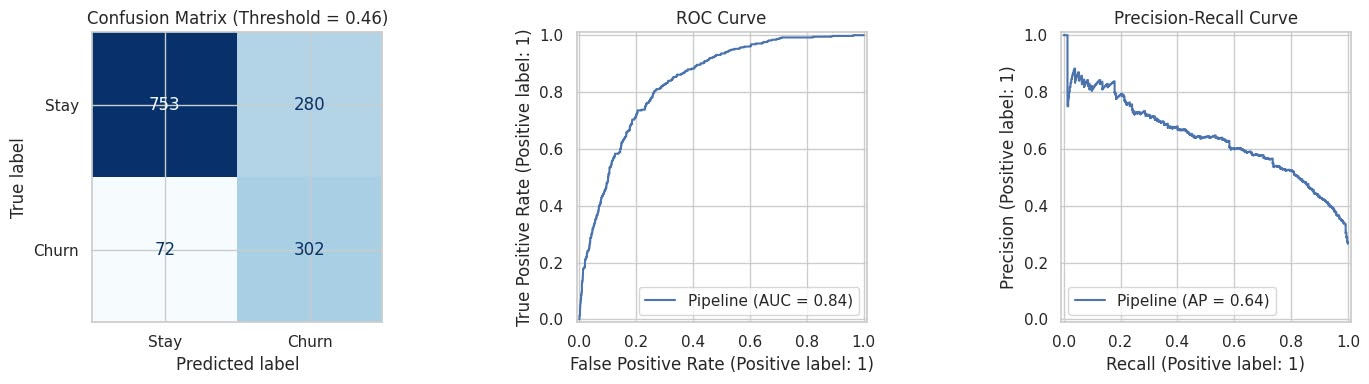
\includegraphics[width=\textwidth]{figure_6_1.png}
\end{center}
\vspace{-0.5em}
\noindent\textbf{Figure 6.1} Confusion matrix (threshold 0.46), ROC curve (AUC = 0.84) and Precision–Recall curve (AP = 0.64) of the tuned Random Forest on the test set (1,407 records).

Key observations:

\begin{itemize}
    \item \textbf{Test performance is consistent with cross-validation.} The test set F1 for the churn class was 0.632, closely matching the 0.636–0.639 range on the training set, indicating no overfitting caused by hyperparameter tuning or threshold selection.
    \item \textbf{Strong churn detection capability.} The model detected 302 out of 374 actual departing customers ($\text{Recall} = 0.807$), missing only 72. ROC-AUC = 0.838 and PR-AUC = 0.639, approximately 2.4 times the random baseline of 0.266.
    \item \textbf{The trade-off is increased false alarms.} Precision = 0.519 implies that only about half of customers flagged as "departed" (302/582) actually departed; 280 staying customers were falsely flagged. The model trades precision for recall, aligning with the asymmetric error costs in Section 5.1.
    \item \textbf{Reduced Accuracy compared to default models (0.750 vs. approx. 0.80)} is a natural consequence of prioritizing minority class Recall rather than a sign of inferiority; this is why accuracy was excluded as the primary metric (Section 4.1.1).
    \item \textbf{The effect of threshold selection is modest.} Lowering the threshold from 0.50 to 0.46 increased Recall by 0.040 (from 0.767 to 0.807), decreased Precision by 0.012, and raised F1 by only 0.004. Most model quality stems from \texttt{class\_weight} rather than thresholding. Comparing both thresholds on the test set is descriptive only, as the 0.46 threshold was decided beforehand on training data.
\end{itemize}

\subsection{ Practical Implications}

The model can be deployed to rank customers by departure probability and target high-risk groups for retention offers. On the test set, out of 582 flagged customers, 302 were genuine churn risks—nearly double the random baseline rate of 26.6% (approx. 374/1,407); thus, model-based targeting achieves nearly twice the precision of random selection (0.519 vs. 0.266).

Retention campaigns are profitable only when expected value from retained customers exceeds incentive costs: if $v$ is remaining customer value, $q$ retention probability, and $c$ incentive cost, offering incentives to a group with Precision $p$ is worthwhile when $p \cdot q \cdot v > c$. Companies must estimate $c$, $q$, and $v$ from real business data to adjust thresholds based on costs rather than F1. EDA findings in Chapter 4 suggest intervention priorities: newer customers (median tenure around 10 months for churners), month-to-month contracts (42.7% churn), and electronic check payments (45.3% churn). These are statistical associations, not causal proofs.

\subsection{ Limitations}

\begin{itemize}
    \item \textbf{Single train/test split and small test set.} With 374 positive samples, metric uncertainty is substantial. Approximate 95% normal-distribution confidence intervals for Recall are roughly 0.77–0.85 and for Precision 0.48–0.56 (excluding threshold-selection effects). Minor performance gaps among models or thresholds should not be interpreted as true underlying differences.
    \item \textbf{Top models are statistically tied.} Random Forest and Logistic Regression differed by only 0.002 in cross-validation F1, well within standard deviation bounds.
    \item \textbf{Small hyperparameter grid.} Only 9 to 27 combinations were tested per model, and boosting models were not evaluated with class weights or stronger variants like XGBoost and LightGBM.
    \item \textbf{Synthetic and cross-sectional data.} The IBM Telco dataset is simulated and cross-sectional, preventing chronological evaluation (training on past data, testing on future) and leaving real-world generalizability unverified.
    \item \textbf{Lack of probability calibration and explainability.} The notebook did not evaluate predicted probability calibration or extract feature importances, leaving key drivers unidentified.
    \item \textbf{F1-optimal threshold assumes equal precision and recall importance}, which may not reflect real cost structures (Section 6.5).
\end{itemize}

\subsection{ Chapter Summary}

On the training set, all models outperformed the baseline, ensemble models and Logistic Regression showed comparable ranking ability (ROC-AUC around 0.85), while Recall at the 0.50 threshold was only around 0.5. Tuning with \texttt{class\_weight = "balanced"} was the most impactful factor for improving F1, bringing Random Forest (cross-validation F1 of 0.636) to the top, closely followed by Logistic Regression (0.634). At a threshold of 0.46, Random Forest achieved a test set Recall of 0.807, Precision of 0.519, F1 of 0.632, ROC-AUC of 0.838, and PR-AUC of 0.639, consistent with cross-validation results.
